\section{Capacity Investment and Transfer Policy}

This section returns to stage 0 and studies how capacity-building policy
affects the equilibrium standardization regime. The key idea is simple:
capacity investment lowers residual compliance costs, and thereby changes the
incentives to form a two-country bloc, to request accession, and to accept
accession.

The results in this section are intentionally more conditional than those in
Sections~3--4. From this point onward, we work with the monotonicity structure
discussed in Appendix~B to ensure that the relevant regime-comparison
functions cross zero in a well-behaved way on an explicit compact parameter
set. Accordingly, the results of Section~5 are local-to-domain comparative
statics established on the verified compact set $\mathcal D'$ reported in
Appendix~B, rather than unrestricted global statements over the entire
admissible set $\mathcal P$.
In particular, the threshold objects used below are established on the
verified compact domain $\mathcal D'$ reported in Appendix~B and rely on two
ingredients: (i) the monotonicity inequalities, which are numerically verified
on $\mathcal D'$, and (ii) the endpoint crossing conditions stated in
Appendix~B.

\subsection{Stage-0 capacity investment}

Recall that participation capacity is given by
\[
\theta_k=\bar\theta_k+I_k,
\qquad
I_k\in[0,1-\bar\theta_k],
\]
and that the residual compliance cost is
\[
\tau_k=\mu(1-\theta_k), \qquad \mu>0.
\]
It is convenient to rewrite this as
\begin{equation}
\tau_k=\bar\tau_k-\mu I_k,
\qquad
\bar\tau_k\equiv \mu(1-\bar\theta_k).
\label{eq:tau_from_x}
\end{equation}

To preserve the symmetry structure of Sections~3 and 4, we focus on symmetric
stage-0 investments by the two high-capacity countries:
\[
I_A=I_B\equiv I_H,
\qquad
\bar\tau_A=\bar\tau_B\equiv \bar\tau.
\]
Hence the post-investment residual costs are
\begin{equation}
\tau=\bar\tau-\mu I_H,
\qquad
\tau_C=\bar\tau_C-\mu I_C.
\label{eq:tau_tauC_from_x}
\end{equation}

Let
\[
R(\tau,\tau_C)\in\{SW,SU,IS\}
\]
denote the equilibrium regime characterized in
Proposition~\ref{prop:regime_choice_main}. At stage 0, government
$H\in\{A,B\}$ and government $C$ choose investments anticipating this regime
map. Their full payoffs are
\begin{align}
\Omega_H(I_H,I_C)
&=
\widehat W_A^{R(\tau,\tau_C)}(\tau,\tau_C)
-\frac{\eta}{2}I_H^2, \label{eq:OmegaH}\\
\Omega_C(I_H,I_C)
&=
\widehat W_C^{R(\tau,\tau_C)}(\tau,\tau_C)
-\frac{\eta}{2}I_C^2, \label{eq:OmegaC}
\end{align}
where $\tau$ and $\tau_C$ are given by \eqref{eq:tau_tauC_from_x}.

Because the regime map is piecewise constant, the stage-0 problem is piecewise
smooth. Inside any region in which the continuation regime is fixed at some
$r\in\{SW,SU,IS\}$, the local investment problem is standard.

\noindent\textbf{Scope of the stage-0 analysis.}
We do not attempt a full global characterization of the simultaneous stage-0
Nash equilibrium across all regime boundaries. The purpose of Section~5 is
narrower: to identify the threshold directions through which capacity
investment shifts regime selection, and to compare the qualitative policy
effects of outsider-side and member-side capacity adjustments on the verified
compact domain reported in Appendix~B.

\begin{lemma}[Local investment condition under a fixed regime]
\label{lem:local_investment_condition}
Fix a regime $r\in\{SW,SU,IS\}$ and suppose that $(\tau,\tau_C)$ lies in the
interior of the region in which $R(\tau,\tau_C)=r$. Then any interior local
optimum of the stage-0 investment problem satisfies
\begin{align}
\eta I_H &= -\mu \frac{\partial \widehat W_A^r(\tau,\tau_C)}{\partial \tau},
\label{eq:FOC_IH}\\
\eta I_C &= -\mu \frac{\partial \widehat W_C^r(\tau,\tau_C)}{\partial \tau_C}.
\label{eq:FOC_IC}
\end{align}
\end{lemma}

\begin{proof}
From \eqref{eq:tau_tauC_from_x}, we have
\[
\frac{\partial \tau}{\partial I_H}=-\mu,
\qquad
\frac{\partial \tau_C}{\partial I_C}=-\mu.
\]
Within a fixed regime $r$, \eqref{eq:OmegaH} and \eqref{eq:OmegaC} are
differentiable, so the first-order conditions are
\[
\frac{\partial \Omega_H}{\partial I_H}
=
\frac{\partial \widehat W_A^r}{\partial \tau}\frac{\partial \tau}{\partial I_H}
-\eta I_H
=
-\mu\frac{\partial \widehat W_A^r}{\partial \tau}
-\eta I_H
=0,
\]
and
\[
\frac{\partial \Omega_C}{\partial I_C}
=
\frac{\partial \widehat W_C^r}{\partial \tau_C}\frac{\partial \tau_C}{\partial I_C}
-\eta I_C
=
-\mu\frac{\partial \widehat W_C^r}{\partial \tau_C}
-\eta I_C
=0,
\]
which gives \eqref{eq:FOC_IH}--\eqref{eq:FOC_IC}.
\end{proof}

Lemma~\ref{lem:local_investment_condition} has an immediate interpretation.
Investment is chosen up to the point where its marginal cost equals the
marginal gain from reducing the relevant residual compliance cost. However,
because the equilibrium regime itself depends on $(\tau,\tau_C)$, governments
may also invest strategically in order to cross a regime boundary.

\subsection{Investment thresholds and regime switching}

The regime conditions in Proposition~\ref{prop:regime_choice_main} can be
translated directly into investment thresholds. To state this cleanly, assume
that the welfare differences in Section~4 satisfy the following monotonicity
property on the relevant domain:
\begin{equation}
\frac{\partial \Delta_A^I}{\partial \tau_C}<0,
\qquad
\frac{\partial \Delta_C^I}{\partial \tau_C}<0,
\qquad
\frac{\partial \Delta_A^{SU}}{\partial \tau}<0,
\qquad
\frac{\partial \Delta_A^{IS}}{\partial \tau}<0.
\label{eq:monotonicity}
\end{equation}

Condition \eqref{eq:monotonicity} says that a higher outsider residual cost
makes accession less attractive both to the outsider and to incumbent members,
while a higher member-country residual cost makes bilateral or full
harmonization less attractive relative to $SW$. Appendix~B verifies these
signs numerically on the broader compact domain
\[
\mathcal D'
=
\left\{
\begin{aligned}
(v,c,\tau,\tau_C):\quad &0 \le v \le 0.055,\\
&0.03 \le c \le 0.06,\\
&0 \le \tau \le 0.04,\\
&0 \le \tau_C \le 0.18
\end{aligned}
\right\}
\subset \mathcal P,
\]
which contains the paper's benchmark numerical examples and a wider range of
baseline trade-cost values.

Under \eqref{eq:monotonicity}, define the accession thresholds
$\tau_C^A(\tau)$ and $\tau_C^C(\tau)$ implicitly by
\begin{align}
\Delta_A^I(\tau,\tau_C^A(\tau)) &= 0, \label{eq:tauCA_def}\\
\Delta_C^I(\tau,\tau_C^C(\tau)) &= 0, \label{eq:tauCC_def}
\end{align}
whenever such roots exist, and define the effective accession threshold
\begin{equation}
\tau_C^{I}(\tau)\equiv \min\{\tau_C^A(\tau),\tau_C^C(\tau)\}.
\label{eq:tauCI_def}
\end{equation}
Likewise, define the member-side formation thresholds $\tau^{SU}(\tau_C)$ and
$\tau^{IS}(\tau_C)$ implicitly by
\begin{align}
\Delta_A^{SU}(\tau^{SU}(\tau_C),\tau_C) &= 0, \label{eq:tauSU_def}\\
\Delta_A^{IS}(\tau^{IS}(\tau_C),\tau_C) &= 0. \label{eq:tauIS_def}
\end{align}

These cost thresholds induce corresponding investment thresholds. In
particular, using \eqref{eq:tau_tauC_from_x}, the minimum outsider investment
required to make accession feasible is
\begin{equation}
I_C^{I}(I_H)
\equiv
\max\left\{
0,\,
\frac{\bar\tau_C-\tau_C^{I}(\bar\tau-\mu I_H)}{\mu}
\right\}.
\label{eq:xC_threshold}
\end{equation}

\begin{proposition}[Capacity thresholds and the equilibrium regime]
Suppose \eqref{eq:monotonicity} holds and the threshold functions defined in
\eqref{eq:tauCA_def}--\eqref{eq:tauIS_def} exist.

\begin{enumerate}
    \item For any given member-country investment $I_H$, accession is feasible
    if and only if
    \[
    I_C \ge I_C^I(I_H).
    \]

    \item If accession is feasible and
    \[
    \Delta_A^{IS}(\bar\tau-\mu I_H,\bar\tau_C-\mu I_C)\ge 0,
    \]
    then the equilibrium regime is $IS$.

    \item If accession is not feasible and
    \[
    \Delta_A^{SU}(\bar\tau-\mu I_H,\bar\tau_C-\mu I_C)\ge 0,
    \]
    then the equilibrium regime is $SU$.

    \item Otherwise, the equilibrium regime is $SW$.
\end{enumerate}
\label{prop:investment_thresholds}
\end{proposition}

\begin{proof}
By Proposition~\ref{prop:regime_choice_main}, $IS$ requires $\Delta_A^I\ge 0$,
$\Delta_C^I\ge 0$, and $\Delta_A^{IS}\ge 0$. Under
\eqref{eq:monotonicity}, the first two inequalities are equivalent to
\[
\tau_C\le \tau_C^A(\tau)
\quad\text{and}\quad
\tau_C\le \tau_C^C(\tau),
\]
which together are equivalent to
\[
\tau_C\le \tau_C^I(\tau).
\]
Using \eqref{eq:tau_tauC_from_x}, this condition becomes
\[
\bar\tau_C-\mu I_C \le \tau_C^{I}(\bar\tau-\mu I_H),
\]
or equivalently
\[
I_C \ge
\frac{\bar\tau_C-\tau_C^{I}(\bar\tau-\mu I_H)}{\mu}.
\]
Imposing the non-negativity constraint on investment yields
\eqref{eq:xC_threshold}. Parts (2)--(4) then follow immediately from
Proposition~\ref{prop:regime_choice_main}.
\end{proof}

Figure~\ref{fig:investment_map} translates the threshold structure of
Proposition~\ref{prop:investment_thresholds} into policy space and shows how
outsider-side and member-side capacity investment move the economy across
regime boundaries.

\begin{figure}[t]
\centering
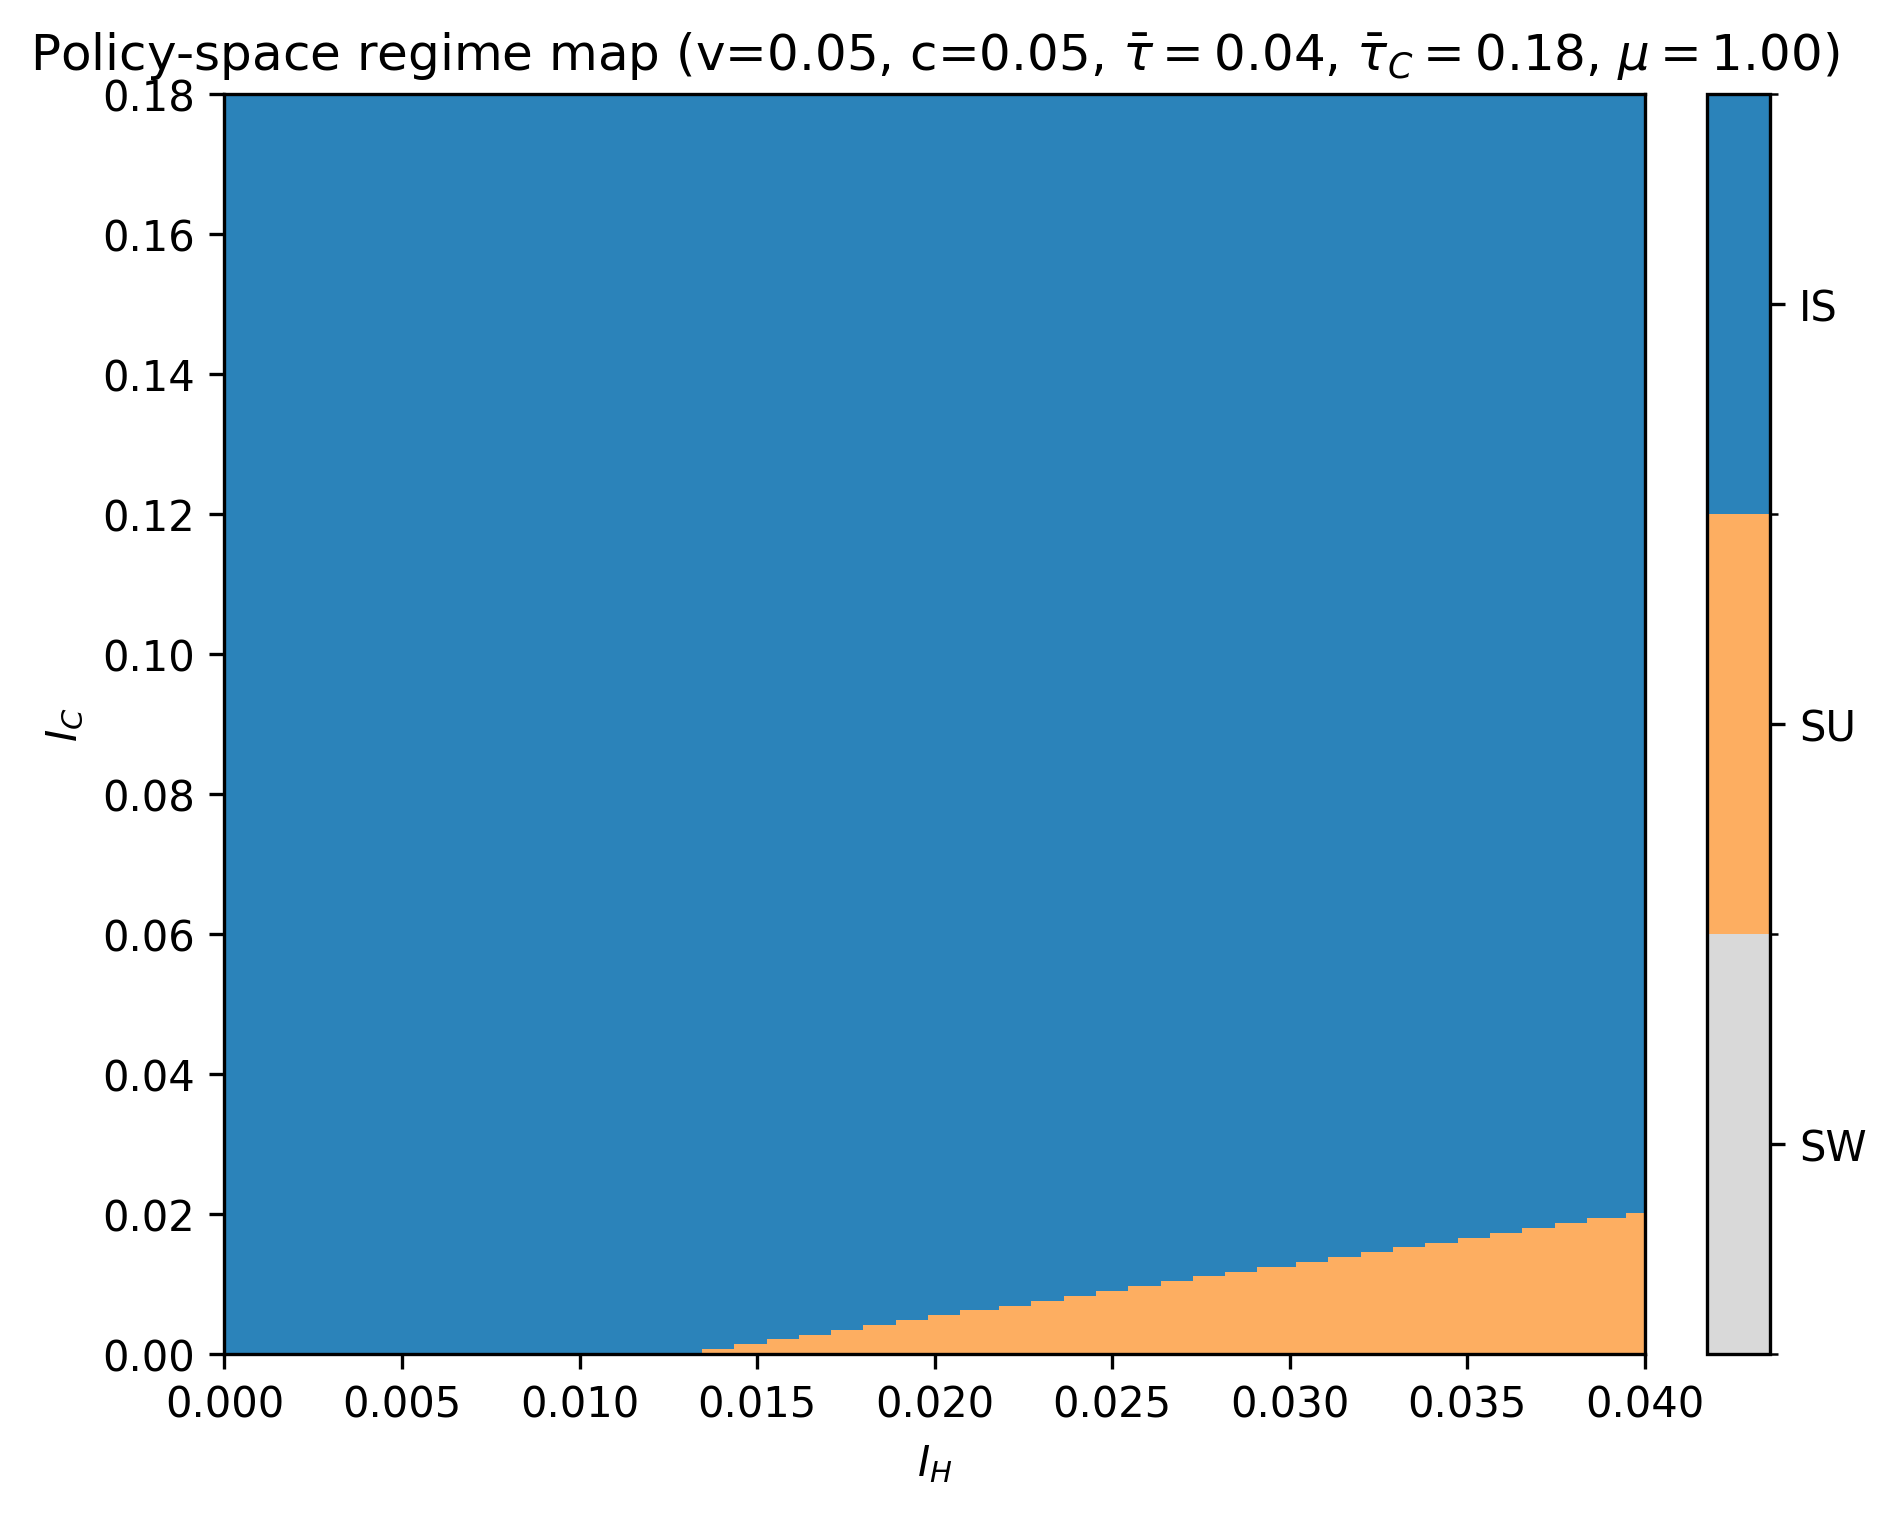
\includegraphics[width=.82\linewidth]{figures/fig4_investment_map.png}
\caption{Policy-space regime map in $(I_H,I_C)$. For fixed primitive parameters $(v,c,\bar{\tau},\bar{\tau}_C,\mu)$, the figure maps the equilibrium regime into the investment space of member-country and outsider-country capacity building. The boundary associated with outsider-side investment captures the effective accession constraint, while the member-side boundary captures the bloc-formation versus harmonization margin emphasized in Proposition~\ref{prop:investment_thresholds}.}
\label{fig:investment_map}
\end{figure}

Proposition~\ref{prop:investment_thresholds} yields a sharp interpretation.
Outsider-side capacity investment mainly relaxes the accession constraint,
while member-side capacity investment mainly relaxes the bloc-formation
constraint. In that sense, the two types of investment operate on different
margins of the regime-selection game.

\subsection{Conditional transfer policy}

Capacity building need not rely exclusively on domestic investment by country
$C$. An international organization, a regional agreement, or the incumbent
member countries may provide technical assistance, certification support, or
conformity-assessment aid. To capture this possibility, suppose that a
conditional transfer $s\ge 0$ can be offered to country $C$.

The transfer is \emph{conditional}: it is implemented only if $IS$ is
realized. Thus, under $IS$, the outsider's effective residual compliance cost
becomes
\begin{equation}
\tau_C^{\,IS}(s)=\tau_C-s,
\qquad
0\le s\le \tau_C,
\label{eq:tauC_transfer}
\end{equation}
whereas payoffs under $SU$ and $SW$ remain unchanged. Let the resource cost of
the transfer be
\begin{equation}
G(s)=\frac{\kappa}{2}s^2,
\qquad \kappa>0.
\label{eq:Gs}
\end{equation}

The transfer $s$ should be interpreted as a reduced-form policy instrument
representing accession-contingent capacity assistance, such as testing support,
certification infrastructure, or implementation aid. The function $G(s)$
captures the real resource cost of providing such support, including
administrative and financing costs. Thus, the policy experiment is not a pure
redistribution exercise, but a stylized way to model costly external support
targeted at the participation bottleneck.

The transfer instrument $s$ is modeled as a planner policy rather than as a
decentralized side payment chosen directly by incumbent member governments. Its
purpose is to capture costly accession-contingent capacity assistance without
embedding a separate bargaining game over who finances the transfer. Modeling
decentralized funding incentives for the transfer is an interesting extension,
but it is outside the scope of the present paper.

Recall the continuation world-welfare measure from
\eqref{eq:world_continuation}:
\[
\widehat W^r(\tau,\tau_C)\equiv 2\widehat W_A^r(\tau,\tau_C)+\widehat W_C^r(\tau,\tau_C).
\]

Because the transfer operates only when $IS$ is implemented, any transfer
level below the accession-enabling threshold is outcome-equivalent to no
transfer at all. Accordingly, the central object is the minimum transfer that
makes accession feasible:
\begin{equation}
s^{acc}(\tau,\tau_C)
\equiv
\max\{0,\tau_C-\tau_C^I(\tau)\}.
\label{eq:sacc}
\end{equation}

The international planner's problem is therefore
\begin{equation}
\max_{s\ge 0}
\left\{
\widehat W^{IS}(\tau,\tau_C-s)-G(s)
\right\}
\quad
\text{subject to }
s\ge s^{acc}(\tau,\tau_C),
\label{eq:planner_transfer}
\end{equation}
with the outside option given by the equilibrium continuation welfare under no
transfer.

\begin{proposition}[Optimal conditional transfer]
Suppose \eqref{eq:monotonicity} holds and $G$ is strictly convex with
$G(0)=0$.

\begin{enumerate}
    \item Any welfare-improving conditional transfer is either zero or at
    least $s^{acc}(\tau,\tau_C)$.

    \item If the optimal transfer is interior and positive, it satisfies
    \begin{equation}
    -\frac{\partial \widehat W^{IS}(\tau,\tau_C-s)}{\partial \tau_C}
    =
    G'(s).
    \label{eq:transfer_FOC}
    \end{equation}

    \item If
    \begin{equation}
    \widehat W^{IS}(\tau,\tau_C-s^{acc})-G(s^{acc})
    \ge
    \max\{\widehat W^{SU}(\tau,\tau_C),\,\widehat W^{SW}(\tau,\tau_C)\},
    \label{eq:transfer_gain}
    \end{equation}
    then there exists an optimal transfer that induces $IS$. Otherwise, the
    planner sets $s=0$ and the no-transfer regime persists.
\end{enumerate}
\label{prop:transfer}
\end{proposition}

\begin{proof}
Part (1) follows directly from the conditionality of the transfer. If
$0<s<s^{acc}$, then accession remains infeasible by \eqref{eq:sacc}, so the
transfer is never implemented. Hence such a transfer is equivalent to $s=0$.

For part (2), conditional on choosing a transfer that induces $IS$, the
planner solves the unconstrained problem
\[
\max_{s\ge s^{acc}}
\left\{
\widehat W^{IS}(\tau,\tau_C-s)-G(s)
\right\}.
\]
The derivative with respect to $s$ is
\[
-\frac{\partial \widehat W^{IS}(\tau,\tau_C-s)}{\partial \tau_C}-G'(s).
\]
Setting this equal to zero gives \eqref{eq:transfer_FOC}.

For part (3), if \eqref{eq:transfer_gain} holds, then the planner weakly
prefers inducing $IS$ with the minimum accession-enabling transfer to any
no-transfer continuation. By strict convexity of $G$, an optimal transfer
exists. If \eqref{eq:transfer_gain} fails, then every transfer that induces
$IS$ yields continuation welfare weakly below the best no-transfer outcome, so
the planner optimally sets $s=0$.
\end{proof}

\subsection{Policy implication}

Proposition~\ref{prop:transfer} clarifies the economic role of transfer policy,
conditional on the verified monotonicity structure imposed above. Standards
fragmentation may persist even when full harmonization is technologically
feasible, because country $C$'s participation capacity is too weak for
accession to be privately attractive. In that case, conditional capacity aid
can restore the missing participation margin directly, rather than trying to
alter the equilibrium indirectly through protectionist standard policies.

The model therefore suggests a conditional policy ranking on the verified
compact domain studied here. When exclusion is driven primarily by
participation-capacity asymmetry, targeted capacity-building measures---such as
technical assistance, testing infrastructure, certification support, or
mutual-recognition implementation aid---are more effective, in the present
framework, at restoring the accession margin than policies that merely
preserve fragmented national standards. In the present framework, the latter
should be interpreted as
policies that maintain the outsider's effective separation from the common
recognition area, rather than as instruments that directly relax the
compliance bottleneck itself.

Finally, the analysis also suggests a reason why decentralized investment may
fall short of what would be desirable from a broader international
perspective. This point should be read as an economic implication of the model
rather than as a separate global theorem. Each government chooses investment
by comparing its own marginal gain with its own marginal cost, as in
\eqref{eq:FOC_IH}--\eqref{eq:FOC_IC}. But accession to a common standard can
create cross-country benefits through market expansion and a larger installed
base, and those gains are not fully internalized by any single government
when investment is chosen non-cooperatively. In that sense, the decentralized
investment benchmark may be too low relative to a coordinated benchmark that
values the full international surplus created by effective accession.
Conditional transfer policy is one possible instrument for narrowing that gap.
